\chapter{Additional data from clonal evolution of microsatellite instability}
\label{app.msiclones}

\begin{figure}[htp]
	\begin{center}
		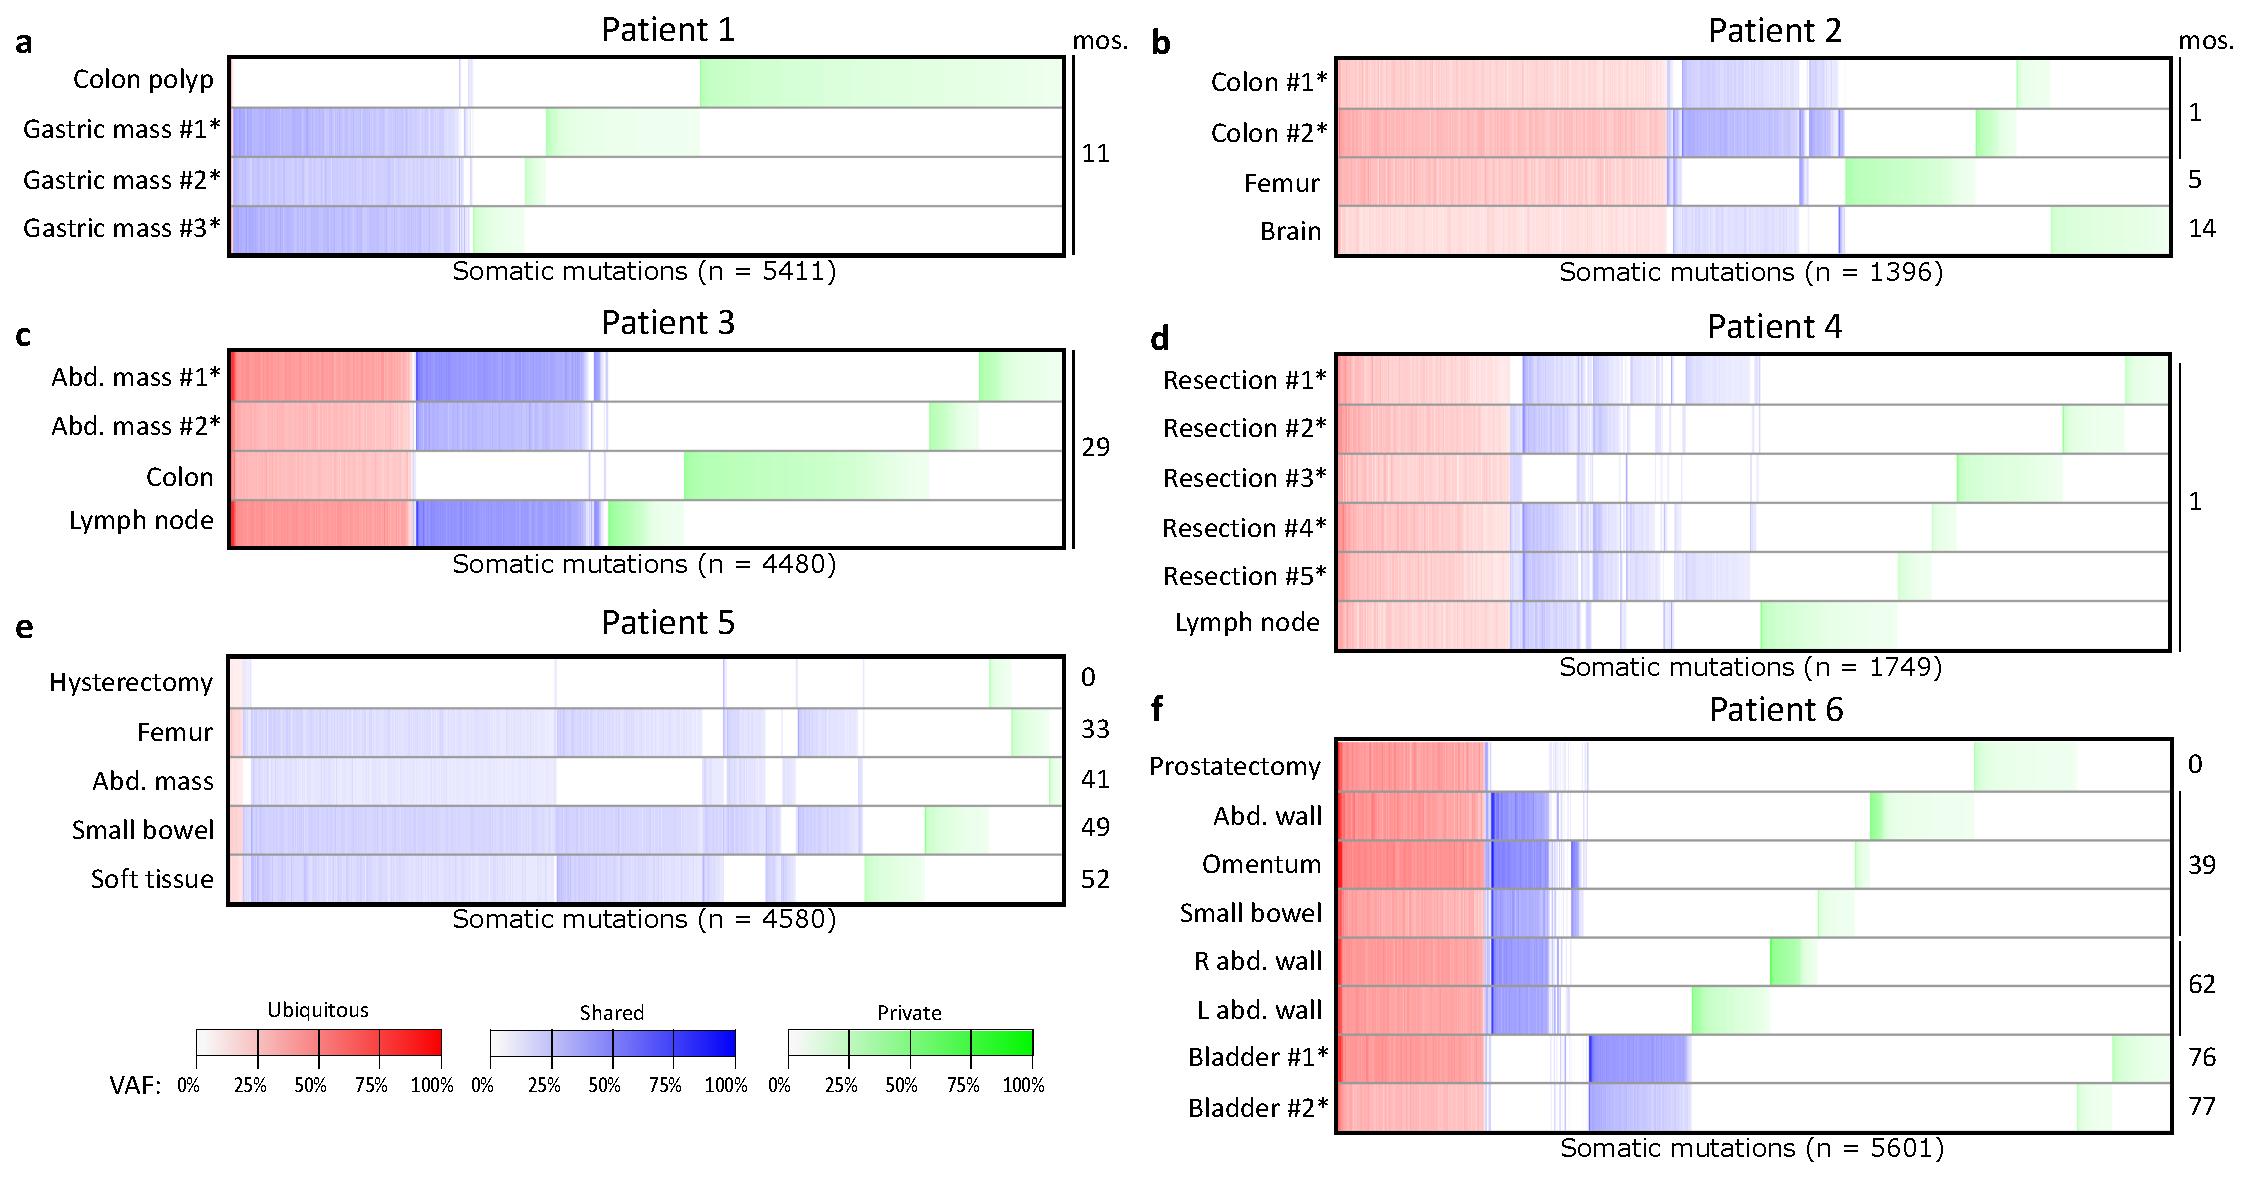
\includegraphics[width=0.98\linewidth]{images/msiclones/supp_mutations_by_sample}
	\end{center}
	\caption[Somatic mutations called with VAF \textgreater{}~6\% in at least one tumor sample.]{Somatic mutation (SNVs and indels) calls with VAF of at least 6\% in tumor samples from six patients with MSI-H cancers \textbf{(a--f)}. Note that in patient 6, bladder \#1 and bladder \#2 were acquired from separate surgeries one week apart. In addition, the colon polyp in patient 1 is believed to have arisen from a separate primary tumor than the gastric mass samples. Within each heatmap, columns in red represent mutations found in all tumor samples, columns in blue represent mutations found in more than one but not all tumor samples, and columns in green represent mutations found in only one tumor sample. Samples marked with asterisks were acquired from a single tumor mass in that patient. mos: months post-diagnosis. Abd: abdominal. VAF: variant allele fraction.}
    \label{fig:msiclones:mutation_heatmaps_min0}
\end{figure}
